% File src/library/utils/vignettes/Sweave.Rnw
% Part of the R package, https://www.R-project.org
% Copyright 2002-2014 Friedrich Leisch and the R Core Team
% Distributed under GPL 2 or later

\documentclass[a4paper]{article}

%\VignetteIndexEntry{Sweave User Manual}
%\VignettePackage{utils}
%\VignetteDepends{tools}
%\VignetteDepends{datasets}
%\VignetteDepends{stats}

\title{Sweave User Manual}
\author{Friedrich Leisch and R-core}

\usepackage[round]{natbib}
\usepackage{graphicx, Rd}
\usepackage{listings}

\lstset{frame=trbl,basicstyle=\small\tt}
\usepackage{hyperref}
\usepackage{color}
\definecolor{Blue}{rgb}{0,0,0.8}
\hypersetup{%
colorlinks,%
plainpages=true,%
linkcolor=black,%
citecolor=black,%
urlcolor=Blue,%
%pdfstartview=FitH,% or Fit
pdfstartview={XYZ null null 1},%
pdfview={XYZ null null null},%
pdfpagemode=UseNone,% for no outline
pdfauthor={Friedrich Leisch and R-core},%
pdftitle={Sweave User Manual},%
pdfsubject={R vignette documentation system}%
}

\sloppy

\usepackage{Sweave}
\begin{document}

\maketitle

\section{Introduction}
\label{sec:intro}

Sweave provides a flexible framework for mixing text and \R{} code for
automatic document generation. A single source file contains both
documentation text and \R{} code, which are then \emph{woven} into a
final document containing
\begin{itemize}
 \item the documentation text together with
 \item the \R{} code and/or
 \item the output of the code (text, graphs)
\end{itemize}
This allows the re-generation of a report if the input data change and
documents the code to reproduce the analysis in the same file that
contains the report. The \R{} code of the complete analysis is embedded
into a \LaTeX{} document\footnote{\url{http://www.ctan.org}} using the
\texttt{noweb} syntax \citep{flm:Ramsey:1998} which is usually used
for literate programming \cite{fla:Knuth:1984}.  Hence, the full power
of \LaTeX{} (for high-quality typesetting) and \R{} (for data analysis)
can be used simultaneously. See \cite{e1071-papers:Leisch:2002} and
references therein for more general thoughts on dynamic report
generation and pointers to other systems.

Sweave uses a modular concept using different drivers for the actual
translations. Obviously different drivers are needed for different
text markup languages (\LaTeX{}, HTML, \ldots). Several packages on
CRAN provide support for other word processing systems (see
Appendix~A).


\section{Noweb files}
\label{sec:noweb}

\texttt{noweb} \citep{flm:Ramsey:1998} is a simple
literate-programming tool which allows combining program source code
and the corresponding documentation into a single file.  A
\texttt{noweb} file is a simple text file which consists of a sequence
of code and documentation segments, called \emph{chunks}:
\begin{description}
\item[Documentation chunks] start with a line that has an at sign
  (\verb|@|) as first character, followed by a space or newline
  character. The rest of this line is a comment and ignored.
  Typically documentation chunks will contain text in a markup
  language like \LaTeX{}.  The chunk continues until a new code or
  documentation chunk is started: note that Sweave does not interpret
  the contents of documentation chunks, and so will identify chunk
  indicators even inside \LaTeX{} verbatim environments.

\item[Code chunks] start with \verb|<<options>>=| at the beginning of
  a line; again the rest of the line is a comment and ignored.
\end{description}
The default for the first chunk is documentation.

In the simplest usage of \texttt{noweb}, the options (if present) of
the code chunks give the names of source code files, and the tool
\texttt{notangle} can be used to extract the code chunks from the
\texttt{noweb} file. Multiple code chunks can have the same name, the
corresponding code chunks are the concatenated when the source code is
extracted. \texttt{noweb} has some additional mechanisms to
cross-reference code chunks (the \verb|[[...]]| operator, etc.),
Sweave does currently not use nor support these features, so they are
not described here.


\section{Sweave files}
\label{sec:sweavefile}

\subsection{A simple example}

Sweave source files are \texttt{noweb} files with some additional
syntax that allows some additional control over the final
output. Traditional \texttt{noweb} files have the extension
\file{.nw}, which is also fine for Sweave files (and fully supported
by the software). Additionally, Sweave currently recognizes files with
extensions \file{.rnw}, \file{.Rnw}, \file{.snw} and
\file{.Snw} to directly indicate a \texttt{noweb} file with Sweave
extensions. We will use \file{.Rnw} throughout this document.

A minimal Sweave file is shown in Figure~\ref{fig:ex1.Rnw}, which
contains two code chunks embedded in a simple \LaTeX{}
document. Running
\begin{Schunk}
\begin{Sinput}
> rnwfile <- system.file("Sweave", "example-1.Rnw", package = "utils")
> Sweave(rnwfile)
\end{Sinput}
\begin{Soutput}
Writing to file example-1.tex
Processing code chunks with options ...
 1 : echo keep.source term verbatim (example-1.Rnw:13)
 2 : keep.source term verbatim pdf  (example-1.Rnw:23)

You can now run (pdf)latex on 'example-1.tex'
\end{Soutput}
\end{Schunk}
translates this into the \LaTeX{} document shown in
Figures~\ref{fig:ex1.tex} and~\ref{fig:ex1.pdf}. The latter can also
be created directly from within \R{} using
\begin{Schunk}
\begin{Sinput}
> tools::texi2pdf("example-1.tex")
\end{Sinput}
\end{Schunk}

The first difference between \file{example-1.Rnw} and
\file{example-1.tex} is that the \LaTeX{} style file
\file{Sweave.sty} is automatically loaded, which provides
environments for typesetting \R{} input and output (the \LaTeX{}
environments \texttt{Sinput} and \texttt{Soutput}). Otherwise, the
documentation chunks are copied without any modification from
\file{example-1.Rnw} to \file{example-1.tex}.

\begin{figure}[htbp]
  \centering
  \begin{minipage}{0.9\textwidth}
    \lstinputlisting{/usr/lib/R/library/utils/Sweave/example-1.Rnw}
  \end{minipage}
  \caption{A minimal Sweave file: \file{example-1.Rnw}.}
  \label{fig:ex1.Rnw}
\end{figure}

The real work of Sweave is done on the code chunks: The first code
chunk has no name, hence the default behavior of Sweave is used, which
transfers both the \R{} commands and their respective output to the \LaTeX{}
file, embedded in \texttt{Sinput} and \texttt{Soutput} environments,
respectively.

The second code chunk shows one of the Sweave extension to the
\texttt{noweb} syntax: Code chunk names can be used to pass options to
Sweave which control the final output.
\begin{itemize}
\item The chunk is marked as a figure chunk (\texttt{fig=TRUE}) such
  that Sweave creates (by default) a PDF file of the plot created by
  the commands in the chunk. Furthermore, a
  \verb|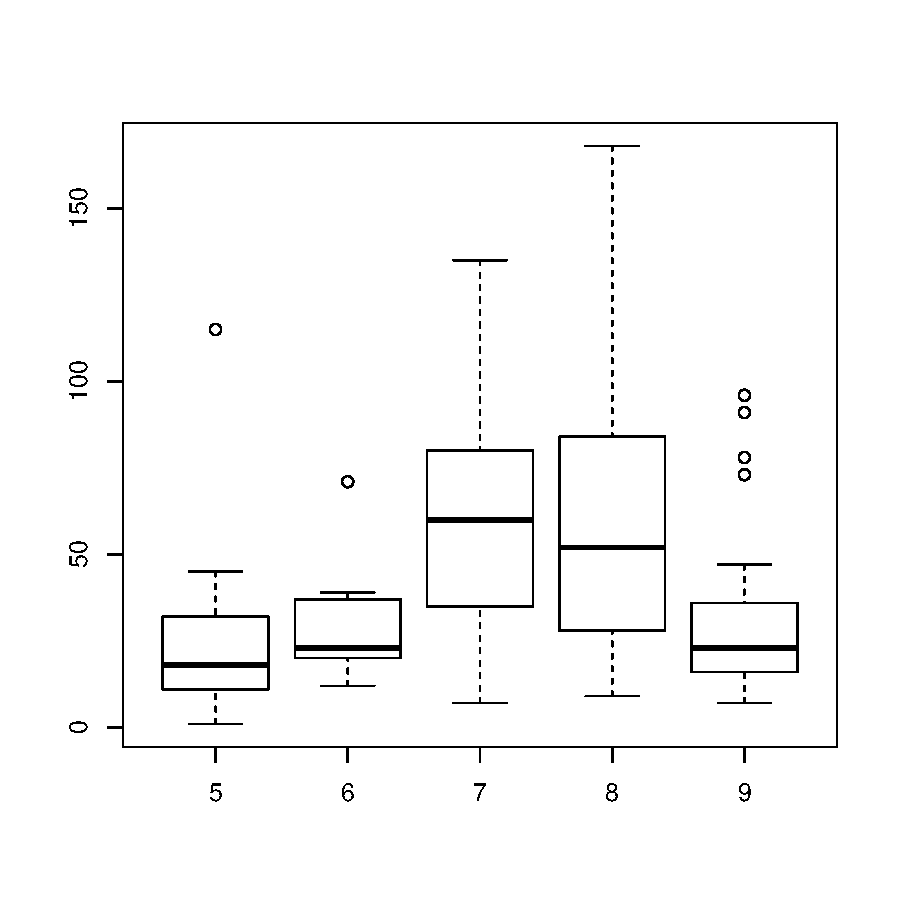
\includegraphics{example-1-002}| statement is inserted into
  the \LaTeX{} file (details on the choice of file names for figures
  follow later in this manual).
\item Option \texttt{echo=FALSE} indicates that the \R{} input should not
  be included in the final document (no \texttt{Sinput} environment).
\end{itemize}

\begin{figure}[htbp]
  \centering
  \begin{minipage}{0.9\textwidth}
    \lstinputlisting{example-1.tex}
  \end{minipage}
  \caption{Running \texttt{Sweave("example-1.Rnw")} produces the file
    \file{example-1.tex}.}
  \label{fig:ex1.tex}
\end{figure}

\begin{figure}[htbp]
  \centering
  \fbox{\begin{minipage}{0.8\textwidth}
    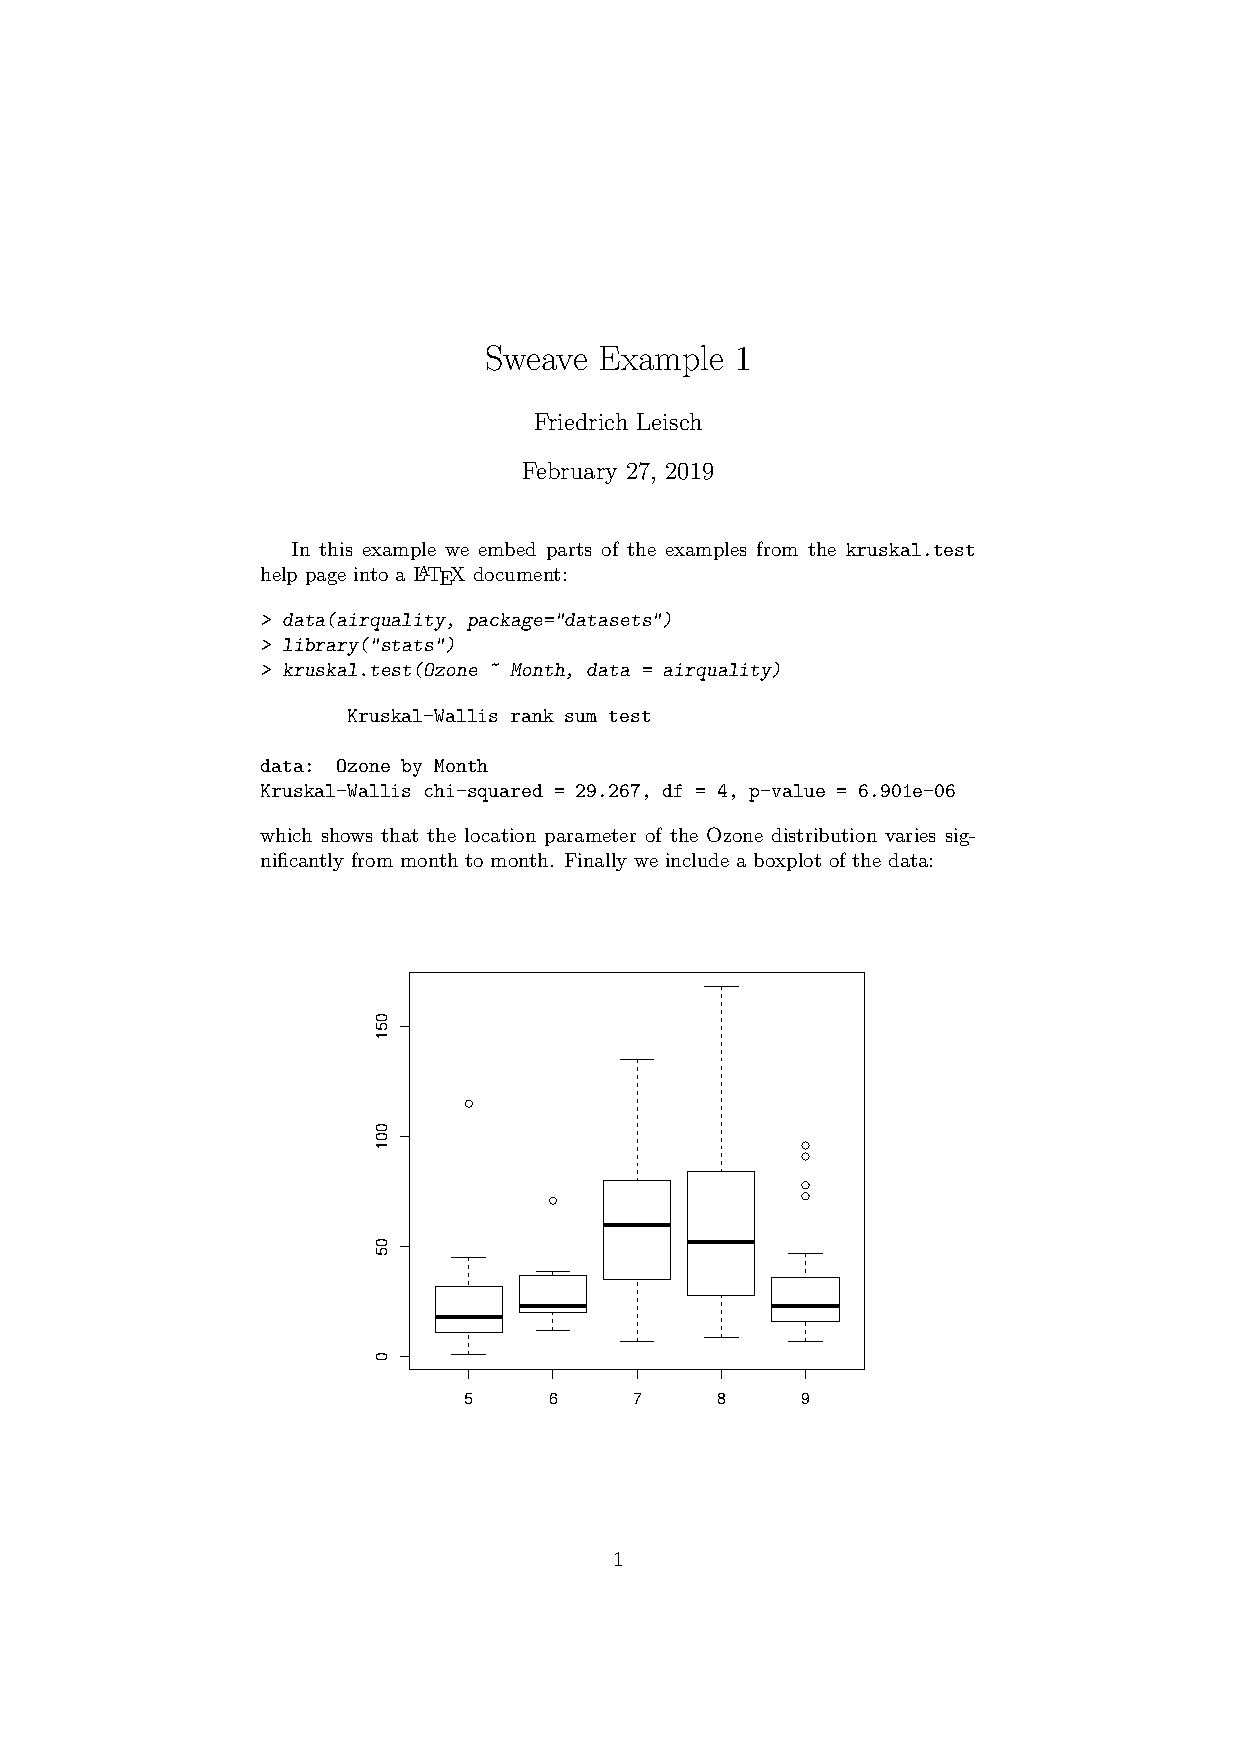
\includegraphics[width=\textwidth]{example-1}
  \end{minipage}}
  \caption{The final document is created by running \texttt{pdflatex} on
    \file{example-1.tex}.}
  \label{fig:ex1.pdf}
\end{figure}


\subsection{Sweave options}

Options control how code chunks and their output (text, figures) are
transferred from the \file{.Rnw} file to the \file{.tex} file. All
options have the form \texttt{key=value}, where \texttt{value} can be
a number, string or logical value.  Several options can be specified at
once (separated by commas), all options must take a value (which must
not contain a comma or equal sign). Logical options can take the
values \texttt{TRUE}, \texttt{FALSE}, \texttt{T}, \texttt{F} as well
as lower-case and capitalized versions of the first two.

In the \file{.Rnw} file options can be specified either
\begin{enumerate}
 \item inside the angle brackets at the beginning of a code chunk,
  modifying the behaviour \emph{only for this chunk}, or
 \item anywhere in a documentation chunk using the command %
  \begin{quote}
    \verb|\SweaveOpts{opt1=value1, opt2=value2, ..., optN=valueN}|
  \end{quote}
  which modifies the defaults for the rest of the document, i.e.,
  \emph{all code chunks after the statement}. Hence, an
  \verb|\SweaveOpts| statement in the preamble of the document sets
  defaults for all code chunks.
\end{enumerate}
Further, global options can be specified (as a comma-separated list of
\texttt{key=value} items) in the environment variable
\verb|SWEAVE_OPTIONS|, and via the \verb|--options=| flag of
\verb|R CMD Sweave|.

Which options are supported depends on the driver in use. All drivers
should at least support the following options (all options appear
together with their default value, if any):
\begin{description}
  \item[split=FALSE:] a logical value. If \texttt{TRUE}, then the output is
   distributed over several files, if \texttt{FALSE} all output is
   written to a single file.  Details depend on the driver.

 \item[label:] a text label for the code chunk, which is used for
   file-name creation when \texttt{split=TRUE}.  It is also used in
   the comments added above the chunk when the file is processed by
   \texttt{Rtangle} (provided the \texttt{annotate} option is true, as
   it is by default), and as part of the file names for files
   generated by figure chunks.

   Because labels can be part of file names, they should contain only
   alphanumeric characters and \texttt{\#+-\_}.  (Including \texttt{.}
   can cause confusion with file extensions.)
\end{description}

The first (and only the first) option in a code chunk name can be
optionally without a name, then it is taken to be a label. I.e.,
starting a code chunk with
\begin{quote}
  \verb|<<hello, split=FALSE>>|
\end{quote}
is the same as
\begin{quote}
  \verb|<<split=FALSE, label=hello>>|
\end{quote}
but
\begin{quote}
  \verb|<<split=FALSE, hello>>|
\end{quote}
gives a syntax error. Having an unnamed first argument for labels is
needed for \texttt{noweb} compatibility. If only \verb|\SweaveOpts| is used for
setting options, then Sweave files can be written to be fully
compatible with \texttt{noweb} (as only file names appear in code chunk
names).

Note that \texttt{split=TRUE} should \textbf{not} be used in package
vignettes.

The help pages for \texttt{RweaveLatex} and \texttt{Rtangle} list the
options supported by the default Sweave and Stangle drivers.

Now for the promised details on the file names corresponding to
figures.  These are of the form \texttt{prefix-label.ext}.  Here
\texttt{prefix} can be set by the option \texttt{prefix.string},
otherwise is the basename of the output file (which unless specified
otherwise is the basename of the input file).  \texttt{label} is the
label of the code chunk if it has one, otherwise the number of the
code chunk in the range \texttt{001} to \texttt{999}.  \texttt{ext} is
the appropriate extension for the type of graphics, e.g.{}
\texttt{pdf}, \texttt{eps}, \ldots{}.  So for the
\file{example-1.Rnw} file, the PDF version of the boxplot is
\file{example-1-002.pdf}, since it is the second code chunk in the
document.  Note that if \texttt{prefix.string} is used it can specify
a directory as part of the prefix, so that for example if
\verb|\SweaveOpts{prefix.string=figures/fig}|, the auto-generated
figures will be placed in sub-directory \verb|figures|: the Sweave
document should arrange to create this before use.

\subsection{Using multiple input files}

\LaTeX{} files can include others via \verb|\input{}| commands.  These
can also be used in Sweave files, but the included files will be
included by \LaTeX{} and are not processed by Sweave.  The equivalent
if you want the included files to be processed is the
\verb|\SweaveInput{}| command.

Included files should use the same Sweave syntax (see below) and
encoding as the main file.


\subsection{Using scalars in text}

There is limited support for using the values of \R{} objects in text
chunks. Any occurrence of \verb|\Sexpr|\verb|{|\texttt{\textit{expr}}\verb|}|
is replaced by the string resulting from coercing the value of the
expression \texttt{expr} to a character vector; only the first element
of this vector is used. E.g., \verb|3| will be replaced
by the string \texttt{'3'} (without any quotes).

The expression is evaluated in the same environment as the code
chunks, hence one can access all objects defined in the code chunks
which have appeared before the expression and were evaluated. The
expression may contain any valid \R{} code, only braces (\verb|{ }|) are
not allowed. (This is not really a limitation because more complicated
computations can be easily done in a hidden code chunk and the result
then be used inside a \verb|\Sexpr|.)

\subsection{Code chunk reuse}

Named code chunks can be reused in other code chunks following later
in the document. Consider the simple example
\begin{quote}% NB: this is indented to avoid interpretation by Sweave.
\begin{verbatim}
 <<a>>=
 x <- 10
 @

 <<b>>=
 x + y
 @

 <<c>>=
 <<a>>
 y <- 20
 <<b>>
\end{verbatim}
\end{quote}
which is equivalent to defining the last code chunk as
\begin{quote}
\begin{verbatim}
 <<c>>=
 x <- 10
 y <- 20
 x + y
 @
\end{verbatim}
\end{quote}

The chunk reference operator \verb|<<>>| takes only the name of the
chunk as its argument: no additional Sweave options are allowed.
It has to occur at the beginning of a line.

References to unknown chunk names are omitted, with a warning.

\subsection{Syntax definition}

So far we have only talked about Sweave files using \texttt{noweb} syntax
(which is the default). However, Sweave allows the user to redefine
the syntax marking documentation and code chunks, using scalars in
text or reuse code chunks.

\begin{figure}[htbp]
  \centering
  \begin{minipage}{0.9\textwidth}
    \lstinputlisting{example-1.Stex}
  \end{minipage}
  \caption{An Sweave file using \LaTeX{} syntax: \file{example-1.Stex}.}
  \label{fig:ex1.Stex}
\end{figure}

Figure~\ref{fig:ex1.Stex} shows the example from
Figure~\ref{fig:ex1.Rnw} using the \texttt{SweaveSyntaxLatex}
definition. It can be created using
\begin{Schunk}
\begin{Sinput}
> SweaveSyntConv(rnwfile, SweaveSyntaxLatex)
\end{Sinput}
\begin{Soutput}
Wrote file example-1.Stex 
\end{Soutput}
\end{Schunk}

Code chunks are now enclosed in \texttt{Scode}
environments, code chunk reuse is performed using
\verb|\Scoderef{chunkname}|. All other operators are the same as in
the noweb-style syntax.

Which syntax is used for a document is determined by the extension of
the input file, files with extension\footnote{or the lowercase
  versions, for convenience on case-insensitive file systems.}
\file{.Rtex} or \file{.Stex} are assumed to follow the
\LaTeX-style syntax. Alternatively the syntax can be changed at any
point within the document using the commands
\begin{quote}
  \verb|\SweaveSyntax{SweaveSyntaxLatex}|
\end{quote}
or
\begin{quote}
  \verb|\SweaveSyntax{SweaveSyntaxNoweb}|
\end{quote}
at the beginning of a line within a documentation chunk. Syntax
definitions are simply lists of regular expression for several Sweave
commands: see the two default definitions mentioned above for
examples.  (More detailed instructions will follow once the API has
stabilized).

\subsection{Encoding}

\LaTeX{} documents are traditionally written entirely in ASCII, using
\LaTeX{} escapes such as \verb|\'e| for accented characters.  This
can be inconvenient when writing a non-English document, and an
alternative input encoding can be selected by using a statement such as
\begin{quote}
  \verb|\usepackage[latin1]{inputenc}|
\end{quote}
in the document's preamble, to tell \LaTeX{} to translate the input to
its own escapes.  There is a wide range of input encodings which are
supported, at least partially, and the more recent \LaTeX{} package
\texttt{inputenx} supports more.  Other encodings commonly encountered
in Sweave documents are \texttt{latin9}, \texttt{utf8} and
\texttt{ansinew} (the CP1252 codepage on Windows).  Greater
coverage\footnote{including Eastern European, Greek and Hebrew
  letters.}  of UTF-8 can be obtained by
\begin{quote}
  \verb|\usepackage[utf8]{inputenx}|
  \verb|\input{ix-utf8enc.dfu}|
\end{quote}

As from \R{} 3.1.0, the UTF-8 encoding is handled preferentially to
other encodings.  Whereas Sweave will convert R code to the local
encoding in general, it leaves UTF-8 code in that encoding, and
outputs in that encoding as well.  Besides the declaration scheme
above, a UTF-8 encoding may be obtained by the \LaTeX{} comment
\begin{quote}
  \verb|%\SweaveUTF8|
\end{quote}

The previous paragraphs covered the documentation sections, but what of
the code sections where \LaTeX{} escapes cannot be used?  The first
piece of advice is to use only ASCII code sections as anything else
will reduce the portability of your document.  But \R{} code can be
included if in the input encoding declared in the preamble.

The next complication is inclusions: the final vignette may well
include \R{} output, \LaTeX{} or other Sweave files \emph{via}
\verb|\input{}| and \verb|\SweaveInput{}| lines, a bibliography and
figures. It is the user's responsibility that the text inclusions are
covered by the declared input encoding.  \LaTeX{} allows the input
encoding to be changed by
\begin{quote}
  \verb|\inputencoding{something}|
\end{quote}
statements: these may not work well in Sweave processing.  Since
\verb|\usepackage[latin1]{inputenc}| is typically not legal \LaTeX{} code
in an included file, it is easiest to declare the encoding to Sweave
using the \verb|%\SweaveUTF8| comment.

It is all too easy for BiBTeX to pick up UTF-8-encoded references for
a Latin-1 document, or \emph{vice versa}.

R output is again to a large extent under the user's control.  If a
Latin-1 Sweave document is processed by \R{} running a Latin-1 locale or
a UTF-8 document is processed in a UTF-8 locale, the only problems
which are likely to arise are from handling data in another encoding,
but it may be necessary to declare the document's encoding to cover
the \R{} output which is generated even if the document is itself ASCII.
One common problem is the quotes produced by \verb|\sQuote()| and
\verb|\dQuote()|: these will be in UTF-8 when \R{} is run in a UTF-8
locale, and will be in CP1252 when Sweave is run from \verb|Rgui.exe|
on Windows.  Two possible solutions are to suppress fancy quotes by
\verb|options(useFancyQuotes=FALSE)| or to force UTF-8 by
\verb|options(useFancyQuotes="UTF-8")|.

The encoding of figures is not usually an issue as they are either
bitmaps or include encoding information: it may be necessary to use
the \texttt{pdf.encoding} Sweave option to set the \texttt{pdf()}
device up appropriately.


\section{Tangling and weaving}

The user front-ends of the Sweave system are the two \R{} functions
\texttt{Stangle()} and \texttt{Sweave()}, both are contained in
package~\pkg{utils}.  \texttt{Stangle} can be used to extract only
the code chunks from an \file{.Rnw} file and write to one or several
files.  \texttt{Sweave()} runs the code chunks through \R{} and replaces
them with the respective input and/or output.  \texttt{Stangle} is
actually just a wrapper function for \texttt{Sweave}, which uses a
tangling instead of a weaving driver by default. See
\begin{Schunk}
\begin{Sinput}
> help("Sweave")
\end{Sinput}
\end{Schunk}
for more details and arguments of the functions.

\subsection{The \texttt{RweaveLatex} driver}

This driver transforms \file{.Rnw} files with \LaTeX{} documentation
chunks and \R{} code chunks to proper \LaTeX{} files (for typesetting both
with standard \texttt{latex} or \texttt{pdflatex}), see
\begin{Schunk}
\begin{Sinput}
> help("RweaveLatex")
\end{Sinput}
\end{Schunk}
for details, including the supported options.

\subsubsection{Writing to separate files}

If \texttt{split} is set to \texttt{TRUE}, then all text corresponding
to code chunks (the \texttt{Sinput} and \texttt{Soutput} environments)
is written to separate files. The file names are of form
\file{prefix.string-label.tex}, if several code chunks have the same
label, their outputs are concatenated. If a code chunk has no label,
then the number of the chunk is used instead. The same naming scheme
applies to figures.  You do need to ensure that the file names
generated are valid and not so long that there are not regarded as the
same by your OS (some file systems only recognize 13 characters).

\subsubsection{\LaTeX{} style file}

The driver automatically inserts a \verb|\usepackage{Sweave.sty}|
command as last line before the \verb|\begin{document}| statement of
  the final \LaTeX{} file if no \verb|\usepackage{Sweave}| is found in
  the Sweave source file. This style file defines the environments
  \texttt{Sinput} and \texttt{Soutput} for typesetting code chunks. If
  you do not want to include the standard style file, e.g., because
  you have your own definitions for \texttt{Sinput} and
  \texttt{Soutput} environments in a different place, simply insert a
  comment like
\begin{verbatim}
% \usepackage{Sweave}
\end{verbatim}
in the preamble of your latex file, this will prevent automatic
insertion of the line.


\subsubsection{Figure sizes}

\file{Sweave.sty} sets the default \emph{\LaTeX{}} figure width (which
is independent of the size of the generated EPS or PDF files).  The
current default is
\begin{verbatim}
\setkeys{Gin}{width=0.8\textwidth}
\end{verbatim}
if you want to use another width for the figures that are
automatically generated and included by Sweave, simply add a line
similar to the one above \emph{after} \verb|\begin{document}|. If you
want no default width for figures insert a
\verb|\usepackage[nogin]{Sweave}| in the header of your file.  Note
that a new graphics device is opened for each figure chunk (one with
option \texttt{fig=TRUE}), hence all graphical parameters of the
\texttt{par()} command must be set in each single figure chunk and
are forgotten after the respective chunk (because the device is
closed when leaving the chunk).

Attention: One thing that gets easily confused are the width/height
parameters of the \R{} graphics devices and the corresponding arguments
to the \LaTeX{} \verb|\includegraphics| command. The Sweave options
\texttt{width} and \texttt{height} are passed to the \R{} graphics
devices, and hence affect the default size of the produced EPS and PDF
files. They do not affect the size of figures in the document, by
default they will always be 80\% of the current text width. Use
\verb|\setkeys{Gin}| to modify figure sizes or use explicit
\verb|\includegraphics| commands in combination with the Sweave option
\texttt{include=FALSE}.

\subsubsection{Prompts and text width}

By default the driver gets the prompts used for input lines
and continuation lines from R's \texttt{options()} settings. To set new
prompts use something like
\begin{verbatim}
options(prompt = "MyR> ", continue = "...")
\end{verbatim}
see \texttt{help(options)} for details. Similarly the output text
width is controlled by option \texttt{"width"}.


\subsubsection{Graphics devices}

The default graphics device for \texttt{fig=TRUE} chunks is
\texttt{pdf()}: the standard options \texttt{pdf}, \texttt{eps},
\texttt{png} and \texttt{jpg} allow one or more of these to be
selected for a particular chunk or (via \verb|\SweaveOpts|) for the
whole document.  It can be convenient to select PNG for a particular
figure chunk by something like
\verb|<<figN, fig=TRUE, pdf=FALSE, png=TRUE>>|: \texttt{pdflatex}
should automatically include the PNG file for that chunk.

You can define your own graphics devices and select one of them by the
option \texttt{grdevice=my.Swd} where the device function (here
\texttt{my.Swd}) is defined in a hidden code chunk. For example, we
could make use of the \texttt{cairo\_pdf} device by
\begin{verbatim}
my.Swd <- function(name, width, height, ...)
  grDevices::cairo_pdf(filename = paste(name, "pdf", sep = "."),
                       width = width, height = height)
\end{verbatim}
Specialized custom graphics devices may need a customized way to shut
them down in place of \verb|graphics.off()|: this can be supplied
\emph{via} a companion function \verb|my.Swd.off|, which is called
with no arguments.

For a complete example see the file
\file{src/library/utils/tests/customgraphics.Rnw} in the \R{} sources.

\subsection{The \texttt{Rtangle} driver}

This driver can be used to extract \R{} code chunks from a \file{.Rnw}
file. Code chunks can either be written to one large file or separate
files (one for each code chunk). The options \texttt{split},
\texttt{prefix}, and \texttt{prefix.string} have the same defaults and
interpretation as for the \texttt{RweaveLatex} driver. Use the
standard \texttt{noweb} command line tool \texttt{notangle} if chunks
other than \R{} code should be extracted. See
\begin{Schunk}
\begin{Sinput}
> help("Rtangle")
\end{Sinput}
\end{Schunk}
for details.

Note that \texttt{split=TRUE} rarely makes much sense, as the files
produced are often interdependent and need to be run in a particular
order, an order which is often not the alphabetical order of the
files.


\section{Adding Sweave Drivers}

Adding drivers is relatively simple by modelling them on\footnote{but
  if you copy, \textbf{do} be careful not to infringe R-core's
  copyright: the copyright notices in the \R{} sources \textbf{must} also
  be copied.} the existing \texttt{RweaveLatex} and \texttt{Rtangle}
drivers.

An Sweave driver is a function of no arguments which should return a
list of five functions:
\begin{description}
\item{\texttt{setup(file, syntax, \dots)}:} Set up the driver, e.g.{}
    open the output file.  Its return value is an object which is
    passed to the next three functions, and can be updated by the next
    two.  The value should be a list, and contain a component
    \texttt{options}, a named list of the default settings for the
    options needed by \texttt{runcode}.
\item{\texttt{runcode(object, chunk, options)}:} Process a code
    chunk.  Returns a possibly updated \texttt{object}.  Argument
    \texttt{chunk} is a character vector, and \texttt{options} is a
    options list for this chunk.
\item{\texttt{writedoc(object, chunk)}:} Write out a documentation
    chunk.  Returns a possibly updated \texttt{object}.
\item{\texttt{finish(object, error)}:} Finish up, or clean up if
    \texttt{error} is true.
\item{\texttt{checkopts(options)}:} Converts/validates \texttt{options}
    given as a named list of character strings.
\end{description}

Note that the \texttt{setup} function should have a \texttt{\ldots}
argument.  It will be passed additional arguments from a
\texttt{Sweave()} call, but in future \texttt{Sweave} may itself set
options and pass them on the setup function: one such may be the
encoding used for the text to be processed.

\bibliographystyle{jss}
\bibliography{Sweave}

\newpage
\appendix


\section{Frequently Asked Questions}
\label{sec:faq}

  \subsection{How can I get Emacs to automatically recognize files
    in Sweave format?}

  Recent versions of ESS (Emacs speaks statistics,
  \url{https://ESS.R-project.org/}) automatically recognize files with
  extension \file{.Rnw} as Sweave files and turn on the correct
  modes. Please follow the instructions on the ESS homepage on how to
  install ESS on your computer.

  \subsection{Can I run Sweave directly from a shell?}

  E.g., for writing makefiles it can be useful to run Sweave directly
  from a shell rather than manually starting \R{} and then running
  Sweave. This can easily be done using
\begin{verbatim}
R CMD Sweave file.Rnw
\end{verbatim}

   % A more elaborate solution which also includes automatically running
   % \texttt{latex} has been written by Gregor Gorjanc and is available
   % at \url{http://www.bfro.uni-lj.si/MR/ggorjan/software/shell/Sweave.sh}.

  \subsection{Why does \LaTeX{} not find my EPS and PDF graphic files when
     the file name contains a dot?}

   Sweave uses the standard \LaTeX{} package \texttt{graphicx} to
   handle graphic files, which automatically chooses the type of file,
   provided the basename given in the \verb|\includegraphics{}|
   statement has no extension.  Hence, you may run into trouble with
   graphics handling if the basename of your Sweave file contains
   dots: \file{foo.Rnw} is OK, while \file{foo.bar.Rnw} is not.

   \subsection{Empty figure chunks give \LaTeX{} errors.}

   When a code chunk with \texttt{fig=TRUE} does not call any plotting
   functions, invalid PDF (or EPS) files may be created. Sweave cannot
   know if the code in a figure chunk actually plotted something or
   not, so it will try to include the graphics, which is bound to
   fail.

   \subsection{Why do R lattice graphics not work?}

   In recent versions of Sweave they do if they would when run at the
   command line: some calls (e.g.{} those inside loops) need to be
   explicitly \code{print()}-ed.

   \subsection{How can I get Black \& White lattice graphics?}

   What is the most elegant way to specify that strip panels are to have
   transparent backgrounds and graphs are to be in black and white when
   lattice is being used with Sweave?  I would prefer a global option that
   stays in effect for multiple plots.

   Answer by Deepayan Sarkar: I'd do something like this as part of
   the initialization:
\begin{verbatim}
 <<...>>
 library(lattice)
 ltheme <- canonical.theme(color = FALSE)     ## in-built B&W theme
 ltheme$strip.background$col <- "transparent" ## change strip bg
 lattice.options(default.theme = ltheme)      ## set as default
 @
\end{verbatim}

  \subsection{Creating several figures from one figure chunk does
     not work}

   Consider that you want to create several graphs in a loop similar
   to
\begin{verbatim}
 <<fig=TRUE>>
 for (i in 1:4) plot(rnorm(100)+i)
 @
\end{verbatim}
   This will currently \textbf{not} work, because Sweave allows
   \textbf{only one graph} per figure chunk. The simple reason is that
   Sweave opens a \texttt{pdf} device before executing the code and
   closes it afterwards. If you need to plot in a loop, you have to
   program it along the lines of
\begin{verbatim}
 <<results=tex,echo=FALSE>>=
 for(i in 1:4){
    fname <- paste("myfile", i, ".pdf", sep = "")
    pdf(file = fname, width = 6, height = 6)
    plot(rnorm(100)+i)
    dev.off()
    cat("\\includegraphics{", fname, "}\n\n", sep = "")
 }
 @
\end{verbatim}


 \subsection{How can I set default \texttt{par()} settings for figure
    chunks?}

  Because Sweave opens a new device for each graphics file in each
  figure chunk, using \texttt{par()} has only an effect if it is used
  inside a figure chunk. If you want to use the same settings for a
  series of figures, it is easier to use a hook function than
  repeating the same \texttt{par()} statement in each figure chunk.

  The effect of
\begin{verbatim}
  options(SweaveHooks = list(fig = function() par(bg = "red", fg = "blue")))
\end{verbatim}
  should be easy to spot.

  \subsection{How can I change the formatting of R input and output
     chunks?}

   Sweave uses the \texttt{fancyvrb} package for formatting all \R{} code
   and text output. \texttt{fancyvrb} is a very powerful and flexible
   package that allows fine control for layouting text in verbatim
   environments. If you want to change the default layout, simply read
   the \texttt{fancyvrb} documentation and modify the definitions of
   the \texttt{Sinput} and \texttt{Soutput} environments in
   \file{Sweave.sty}, respectively.


  \subsection{How can I change the line length of R input and
     output?}

   Sweave respects the usual way of specifying the desired line length
   in R, namely \texttt{options(width)}. E.g., after
   \texttt{options(width = 40)} lines will be formatted to have at most 40
   characters (if possible).


  \subsection{Can I use Sweave for Word files?}

  Not directly, but package~\pkg{SWord} provides similar
  functionality for Microsoft Word on Windows platforms.

  \subsection{Can I use Sweave for OpenOffice files?}

   Yes, package \CRANpkg{odfWeave} provides functions for using Sweave in
   combination with OpenOffice Writer rather than \LaTeX.

   \subsection{Can I use Sweave for HTML files?}

   Yes, package \CRANpkg{R2HTML} provides a driver for using Sweave in
   combination with HTML rather than \LaTeX.

   \subsection{After loading package \pkg{R2HTML} Sweave doesn't
     work properly!}

   Package \CRANpkg{R2HTML} registers an Sweave driver for HTML files
   using the same file extensions as the default \texttt{noweb}
   syntax, and after that its syntax is on the search list before the
   default syntax.  Using
\begin{verbatim}
  options(SweaveSyntax = "SweaveSyntaxNoweb")
\end{verbatim}
or calling Sweave like
\begin{verbatim}
  Sweave(..., syntax = "SweaveSyntaxNoweb")
\end{verbatim}
ensures the default syntax even after loading package \CRANpkg{R2HTML}.

\end{document}

%%% Local Variables:
%%% mode: latex
%%% TeX-master: t
%%% End:
